%\addcontentsline{toc}{chapter}{Development Process}
\chapter{Design}
This chapter will discuss the overall architecture and higher level aspects of the platform's design. It is only intended to provide an overview of the design. A more in-depth discussion of specific design decisions will be presented on a per-iteration basis later in the report.

\section{Overall Architecture}
The platform is comprised of 3 key systems: a REST API that interfaces with a MongoDB database; an Android App to consume the API and serve content to Customers and Drivers; a Responsive Web App to consume the API and serve content to Company Admins. The overall architecture of the system can be seen in Figure~\ref{fig:overall_architecture}.

Both the Android and Web App are categorized as user-facing systems. Meaning the platform's users are never intended to interact with the API directly, but rather through one of these two Applications (depending on their role). This also means that the two user-facing  Applications never interact with each other, they exclusively send and receive data from the API.

Data received from the API is in JSON format, which is natively deserialized by Javascript and Typescript. However, Android's GSON library is used to support JSON conversion to and from 'plain old Java objects' (POJOs).

\newpage

\begin{figure}[!htb]
	\centering
	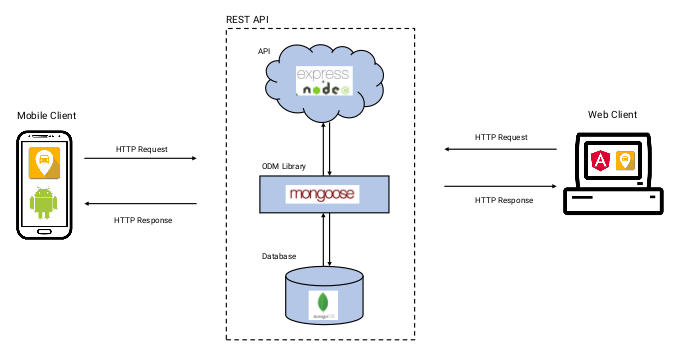
\includegraphics[width=0.75\linewidth]{Resources/img/overall_architecture.png}
	\caption{The Overall Architecture of the Platform}
	\label{fig:overall_architecture}
\end{figure}

\begin{figure}[!htb]
	\centering
	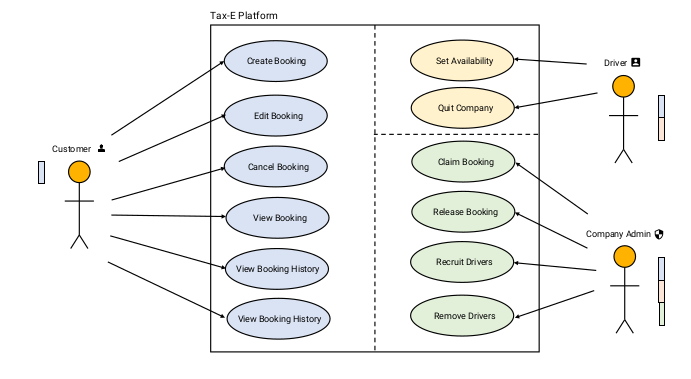
\includegraphics[width=0.75\linewidth]{Resources/img/overall_use-case.png}
	\caption{The Use-Cases of the Platform for each User type}
	\label{fig:overall_use-case}
\end{figure}


\section{REST API Architecture Overview}
Broadly, the REST API is a modular system split up into the following: models, services, controllers, routes, middlewares, and helpers.

The model module contains all the models for the system. These directly map onto a collection within the MongoDB database. Some models may reference each other using MongoDB ObjectIDs, comparable to SQL's foreign key constraint. Any model file can be referenced from anywhere within the system and used as a 'type' to initialize objects.

The services module is the lowest level of abstraction for interfacing with the backend database. It exposes several necessary public functions to the rest of the system. Typically, it will implement CRUD functions via mongoose. The service files are only intended to be accessible from their respective controllers.

Controllers are the next level up from services in the API's abstraction layers. Controller files are called by the API's router to pass information from the HTTP request to the required service. Then execute the relevant middleware. The functions within a controller file are typically very simple and simply serve as an intermediary between the router and the services themselves.

Routes are used to capture information from the HTTP request and pass it to the controllers so the relevant operations can be completed (via the service).  These include retrieving values from request headers, the request body, and any URL parameters or queries. The various layers of abstraction within the API can be seen in Figure~\ref{fig:abstraction_layers}

\begin{figure}[!htb]
	\centering
	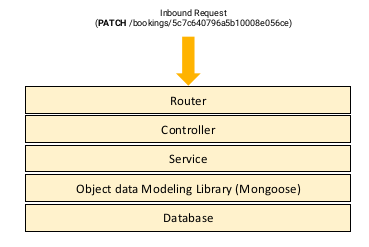
\includegraphics[width=0.75\linewidth]{Resources/img/abstraction_layers.png}
	\caption{The layers of abstraction within the API.}
	\label{fig:abstraction_layers}
\end{figure}

Several middleware files were created for the API, middleware is executed by the router before any code from the controller is executed. Middleware can be configured to run on every route or to be executed on a per-route basis. For example, the error handling middleware needs to be executed on every route. However, a piece of middleware such as access control or authentication may only need to be executed on certain protected routes. The order of execution of middleware for a route that requires every piece of middleware is depicted in Figure~\ref{fig:middleware}.

\newpage

\begin{figure}[!htb]
	\centering
	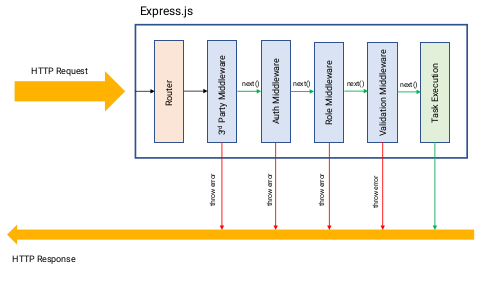
\includegraphics[width=0.75\linewidth]{Resources/img/middleware.png}
	\caption{Diagram to display the order of execution of middleware.}
	\label{fig:middleware}
\end{figure}

Helpers do not have a designated place in the order of execution of requests. Rather, they are intended to be used by other modules within the API to perform frequent, utility tasks or to enumerate types. For example, there are two enumeration types within the helper module 'role' and 'status'. These are used across many different modules within the API to reduce code duplication.

\section{Data Model}
The data model for the platform is fairly straight forward, the simple, flexible nature of MongoDB certainly assisted in this simplicity. To preface, a 'collection' in this context is comparable to a 'relation' in a traditional relational DBMS. A 'document' is comparable to a 'tuple' or 'record', and a 'field' is comparable to a 'column' or 'attribute'.

The data model contains three collections 'User', 'Booking', and 'Company'. All collections have unique Object IDs and each collection references another. The 'User' collection is likely the largest, it is a general model for Customers, Drivers, and Company Admins. The decision to use a single, larger model for all users, as opposed to a specific model for each type of user was made early on, due to its simplicity. This is implemented by leaving the type-specific fields as null if they are not applicable to the user. A user's type is stored using the 'role' field. The data model is depicted in the Entity Relationship seen in Figure~\ref{fig:entity_relationship}.

\newpage

\begin{figure}[!htb]
	\centering
	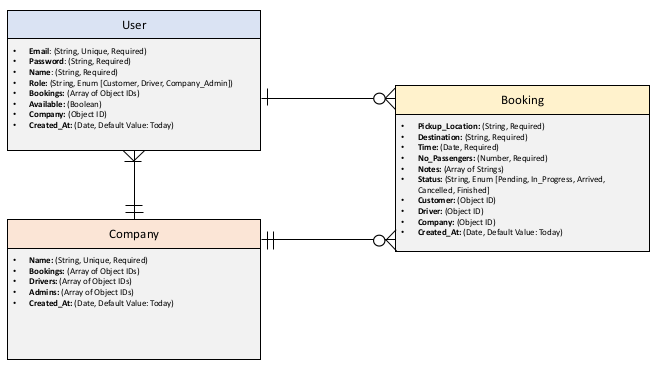
\includegraphics[width=\linewidth]{Resources/img/entity_relationship.png}
	\caption{An Entity-Relationship diagram to accurately depict the Data Model used }
	\label{fig:entity_relationship}
\end{figure}

\section{Android App Architecture Overview}
Much of the Android App's design is boilerplate, with the main package split into java code and app resources. There are no significant differences between the app's build variants as it is intended to offer different functionality dynamically, depending on the user's role. It was considered early on to provide two different variants of the app, one for customers and another for drivers. However, as the differences between the two app's functionalities would be very minor it was decided that a single app would be the best approach.

The app's main java package is comprised of five sub-packages: model, network, ui, util, and viewmodel.

The model package contains 5 model classes, each representing a type of JSON response that can be received from the API. They are required to enable serialization/de-serialization of JSON objects. The 'User', 'Booking', and 'Company', and 'Response' models are the ones uses most frequently. With 'LoginResponse' only being used in a single special case. The Response model is returned anytime the API is expected to return a generic response with no particularly important data. It is very useful for Error Handling for retrieval of JSON values.

The network package contains the classes required to interface with the API using Retrofit. It contains the 'RetrofitInterface' interface, which is comparable to the Repository interface that would be used in Android's data persistence library. The 'NetworkUtil' class has several overloaded methods that each return a differing instance of the RetrofitInterface. For example, if the method is called with no parameters it returns a Retrofit instance with no HTTP authentication headers. Whereas, if the method is called with an access token as a parameter, it returns a Retrofit instance with the access token in the HTTP headers.

All of the app's activity and fragment classes are located in the ui package. The package itself is split into 5 sub-packages, which are intended to relate to each of the app's screens and dialogs. The app has two main activities Authentication and Main. This is how access control is enforced in the app, the user can only access the main activity if they have successfully logged in via the authentication activity. There are of course other activities within the app, but they are always called on top of one of the two main activities.

The util package contains all of the classes that contain shared code that is intended to be used all across the app. This includes the app's error handler, validator, shared preference manager, customer de-serializers, enum types, and more. The use of a util package with these classes is intended to reduce code duplication.

The Model View ViewModel (MVVM) design pattern is implemented in this app via the viewmodel package. The view models within this package provide a layer of abstraction between the networking and UI classes. In the case that the API's routes were updated, supporting this update in the app is made considerably easier using view models. Therefore increasing maintainability and encouraging good object orientation practices.

\section{Web App Architecture Overview}
The Web Application is likely the simplest system within the platform. Similarly to the Android Application, the main directories are fairly similar to a boilerplate Angular Application. The main directory of the app contains seven sub-directories: '\_guards', '\_helpers', '\_models', '\_services', 'components', 'layouts', 'modules'.

The '\_guards' directory currently contains a single guard file to enforce authentication within the app.

The '\_helpers' directory contains two HTTP interceptors, an error interceptor, and an access token interceptor. The error interceptor is intended to intercept incoming responses from the API and handle any errors appropriately. If the application was of a larger scale, it would likely be more appropriate to also have a designated error handling file. However, due to the scale of the application currently, this solution was selected due to its simplicity. The 'jwt' interceptor is intended to intercept outgoing requests to the API and append the user's access token to the request headers. This means that the token doesn't have to be manually added each time a request is made.

The '\_services' directory contains all of the services required by various views. The services are intended to add a layer of abstraction between the view and the HTTP requests. There is also a service file for displaying notifications in the view, it works by injecting a HTML element into the view and running jQuery code to animate the element.

All of the app's angular components reside in the 'components' directory. An angular component represents a 'page' within the app, with components belonging to a module. For example, the 'drivers' page is a component that belongs to the 'main' module. Each component contains a view file, style file, and controller file. These are typically html, scsss, and typescript files respectively.

Any recurring layouts within the app reside in the 'layouts' directory. This includes things such as headers, footers, navbars, etc. Similarly to components, each layout has a view, style, and controller file. However, the layout directory is treated as its own Angular module.

Lastly, the modules directory contains the app's two main modules 'auth' and 'main', these modules create a scope in which components can exist. Each module requires a router and module file, in addition to the files required by standard components. A module's view file will typically contain a placeholder for whichever component the module's router serves.

\section{User Interface}
The User Interface for both the Android Application and the Responsive Web Application is intended to conform to Google's Material Design guidelines~\cite{material_documentation_ref}. By attempting to implement Material Design in all of the platform's user-facing applications, a consistent and familiar style is created. Together with a consistent colour scheme and typeface, it strives to provide the best user experience.

Implementing Material Design in the Android Application was made trivial with the tools that Android Studio provides. Once a colour scheme was selected, the hex values were simply entered into the App's relevant resource file. Any components subsequently created were coloured accordingly. A bottom navigation bar was used for the app's main navigation, the bar is rendered differently depending on the user's role.

Due to time restrictions, a third party UI template was used for the Web App. The template, 'Material Dashboard Angular'~\cite{angular_material_documentation_ref}, uses Bootstrap, Sass, and HTML5 to create a productivity dashboard template that conforms to Google's Material Design. The template also provides some boilerplate Angular files for routing and layout displays, these were adapted from the provided code for the needs of the application.

\begin{figure}[!htb]
	\centering
	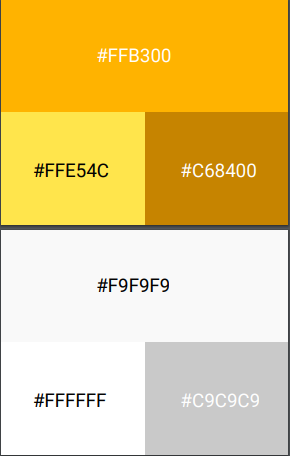
\includegraphics[width=0.25\linewidth]{Resources/img/color-scheme.png}
	\caption{The Colour Scheme Selected for the Platform}
	\label{fig:color-scheme}
\end{figure}

\section{Technologies Used}
As the developed platform would contain several systems, it was clear that a diverse array of technologies would need to be adopted. Both to aid project management and for use in implementation. This section will discuss the selected technologies for this project.

\subsection{Implementation}
With regards to the technology that would be used to develop the REST API, it was a close decision between Rails 5 and Node.js / Express.js. Although Flask and ASP.net were most certainly fit for purpose and had plenty of documentation to get started. There was a distinct lack of experience in the underlying languages (Python \& C\#). The project supervisor had a level of expertise in Rails, this would have been an advantage for the adoption of this framework. However, due to personal preference and a slight bias towards Javascript, Node.js together with Express.js was selected. This choice showed great promise, with a considerable amount of online resources and available testing libraries. It would also mean the development of the API would integrate seamlessly with Node.js's default package manager (NPM). This would allow access to hundreds of thousands of javascript packages.

Having researched both Angular and React it was clear they were both equally appropriate for this task. However, Angular's traits were increasingly more appealing after in-depth research. It offered a substantial amount of in-built functionality compared to React. Examples of these functionalities are an In-built XSS protection, a native Router (eliminating the need for a third party library), a form builder, and SCSS compiling. It also supported Google's Material Design, through pre-built components, this was ideal to ensure consistency between the platform's applications. The only considerable drawback was that Angular is based in Typescript, a syntactically strict superset of Javascript; this was an unfamiliar technology. However, given the considerable advantages and previous experience with Javascript, the benefits certainly outweighed the drawbacks. It should also be mentioned that the adoption of Angular would loosely complete the project's adoption of the MEAN stack~\cite{mean_documentation_ref}.

\subsection{Data Persistence}
Although the research was certainly a key part of making a fully informed decision; a JSON-like document-oriented DBMS seemed like an obvious fit, having already decided to use Node.js for the API. Therefore, MongoDB was selected.  One disadvantage of a NoSQL solution is that complicated queries are typically considered more difficult compared to a traditional SQL DBMS. However, given the simple nature of the queries for this project, this didn't seem overly relevant. 

\subsection{Development Environments}
Having researched JetBrains' WebStorm, it was decided it would be a better fit for the development of both the platform's REST API and Web Application. With substantial language-specific support, code completion, syntax highlighting, and a preview of markdown files, it was an easy decision. WebStorm also provides in-built integration with docker, GitHub, and NPM.

\subsection{Project Management}
After researching many project management solutions, a decision was made to use Docker for containerization of the REST API. This conclusion was mainly motivated by the ability to easily replicate the development environment across multiple machines. Due to Extreme Programming being the project's chosen development methodology, a Continuous Integration tool had to be selected. Having researched several options, it was eventually decided that TravisCI would be used. It was by far the most lightweight and easy to understand tool of those researched. It seamlessly integrates with GitHub through the use of a single YAML file and OAuth, making adoption relatively easy for inexperienced users.

\subsection{Deployment}\label{deployment}
In order to make an informed decision regarding the deployment method for the API and Web Application, sample applications were deployed using both Heroku and AWS. It was discovered that the process was actually a lot more in-depth than initially anticipated. Together with having to register an account and provide banking details this was somewhat discouraging. Therefore the API and Web Application were both deployed to a home-based headless ubuntu-server box. The API is deployed using Nginx as a reverse proxy and Node.js's process manager, PM2. The Web Application is deployed using an Apache web server.

Although there are certain security implications with a 'homemade' deployment solution.  For example, the lack of reliable SSL encryption and physical security concerns due to the location of the server itself. The deployment is only intended for demonstration purposes and will likely only contain fictitious test data. If the platform were ever to be deployed for production, a fully supported commercial solution would be sought out.




